%\documentclass[tikz,border=5mm,convert={outfile=\jobname.png}]{standalone}
\documentclass[tikz,border=5mm]{standalone}
\usepackage[utf8]{vietnam}
\usepackage{tikz}
\usetikzlibrary{calc}
\begin{document}
	%==================
	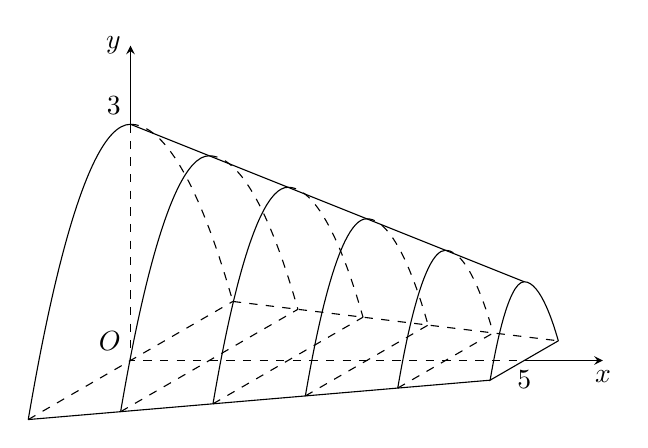
\begin{tikzpicture}
		\def\g{30}%Góc này có thể thay đổi để thay đổi độ nghiêng của hầm.
		\def\f(#1){3-#1 *2/5}%Hàm số chiều cao hầm
		\pgfmathsetmacro{\hm}{\f(0)}
		\pgfmathsetmacro{\xm}{\hm *cos(\g)/2}
		\pgfmathsetmacro{\ym}{\hm *sin(\g)/2}
		\pgfmathsetmacro{\hh}{\f(5)}
		\pgfmathsetmacro{\xh}{\hh *cos(\g)/2}
		\pgfmathsetmacro{\yh}{\hh *sin(\g)/2}
		\draw[dashed] (\xm,\ym)--(5+\xh,\yh);
		\draw[dashed] (0,\hm)node[above left]{$3$}--(0,0)node[above left]{$O$}--(5,0)node[below]{$5$};
		\draw[-stealth] (0,\hm)--(0,\hm+1)node[left]{$y$};
		\draw[-stealth] (5,0)--(6,0)node[below]{$x$};
		\draw (0,\f(0))--(5,\f(5));
		\draw (-\xm,-\ym)--(5-\xh,-\yh);
		\draw (5-\xh,-\yh) parabola bend (5,\hh) (5+\xh,\yh)--cycle;
		\foreach \i in {0,...,4}{
			\pgfmathsetmacro{\h}{\f(\i)}
			\pgfmathsetmacro{\x}{\h *cos(\g)/2}
			\pgfmathsetmacro{\y}{\h *sin(\g)/2}
			\draw[dashed] (\i,\h) parabola (\i+\x,\y);
			\draw (\i,\h) parabola (\i-\x,-\y);
			\draw[dashed] (\i-\x,-\y)--(\i+\x,\y);
		}
	\end{tikzpicture}
\end{document}